This section describes the overview of the SmartRobotinoInstructionPlanner component. The major use-case of this component is described and how it works together with other components. Also it is described which problems occurred during the development of it and how they were solved. 


\subsubsection{Overview}
\label{sec:inst_overview}

The SmartRobotinoInstructionPlanner component is responsible for the task coordination between the components used in the software written for the 
Robocup Logistics League. This component was introduced by the previous team of master students in 2016. The intention behind this component was the scenario was made out of a master robot and various slave robots. The master robot should process the information received from the Robocup Logistics Referee Box and start instructing the slaves on the field. Therefore this component should only run on the master robot. \\

Various features like driving around the field or detecting MPS stations is implemented in other components but not in the SmartRobotinoInstructionPlanner component. For instructing these components a task sequencer (which is called SmartLispServer and was provided by the SmartSoft team). To instruct these components by the sequencer, task blocks need to be written in a language called SmartTCL. This language is based on Common Lisp and was developed inside the ZAFH lab of the University of Applied Sciences Ulm \cite{SS10}.  \\ 

The SmartRobotinoInstructionPlanner is connected to the RefboxServer component using two SmartSoft ports. One port is for transmitting messages from the Referee Box to the Instruction Planner and the other is for sending information about detected MPS stations back to the Referee Box. For sending information between those two components, special communication objects are used which makes it easier to parse and process those messages. These messages need to be written in a special DSL for communication objects and are later converted to C++ classes. Using these classes those messages can be easily processed within those components \cite{CO}. \\


\begin{figure}[h]
\centering
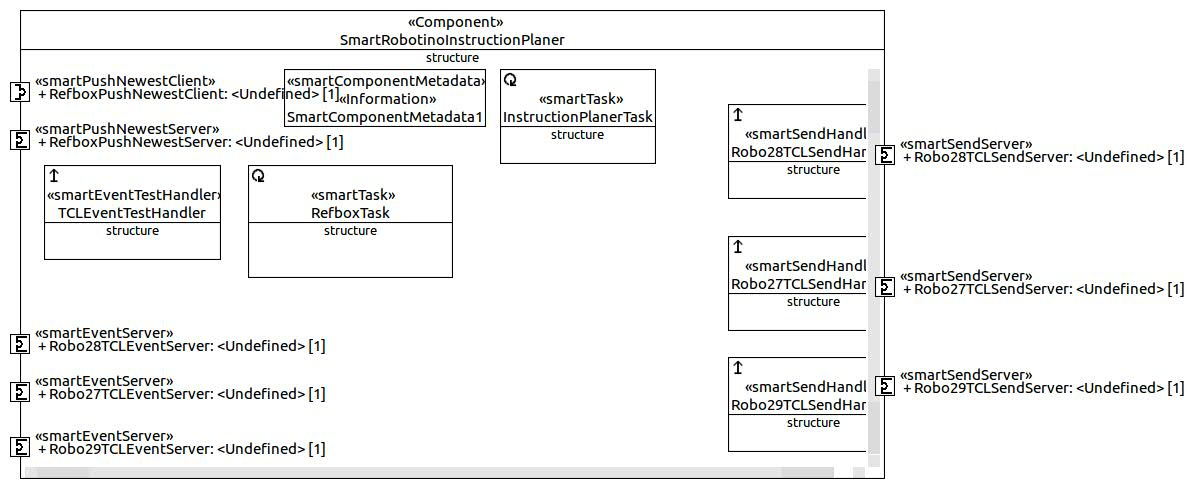
\includegraphics[scale=0.25]{pic/SmartRobotinoInstructionPlaner.JPG}
\caption{Model of Instruction Planner}
\label{fig:i_overview}
\end{figure}


Figure \ref{fig:i_overview} shows the SmartSoft model of the Instruction Planner. Various message ports can be seen on the outside of the component. These are the communication ports between the Instruction Planner and the RefBoxServer, but also the SmartLispServer. Also two SmartTask can be seen which are used to implement message processing between those components. The RefboxTask handles all the messages which are send from the RefboxServer component to the Instruction Planner. The InstructionPlannerTask has more importance than the RefboxTask for the Instruction Planner. In this task the whole message processing between the Referee Box and the Robotino and the messages between other components and the Instruction Planner is done. \\


In the 2016 design of the Instruction Planner the master robot expected a list of possible zones from the Referee Box when the exploration phase starts. In these possible zones, possible MPS stations of the team can be located. It was intended that a master robot should process this list of zones and splits this list up into three equal parts. These parts can then be deployed on all Robotinos for exploring the field. This enabled a concurrent exploration of the field by all three Robotinos.  Unfortunately in 2017 the Robocup Logistics League committee removed the list of possible zones from the rules to make it harder for the teams to archive a successful exploration phase \cite{RC17}. Therefore the intentional implementation has no function anymore and needed to be adapted to the new rules. So the functionality of the Instruction Planner shifted more into the overall task combination instead of only splitting the list of possible zones into equal parts. \\



\subsubsection{Previous implementation}
\label{sec:previous}

As described in \cite{BOK} the Instruction Planner was designed for planning and coordination of other components on the master and the slave Robotinos. This means that it was designed that on all slave robotinos only the necessary parts like driving, detection or docking should run. All coordination should be done by the Instruction Planner on the master robotino. To show the difference between the 2016 version and the 2017 version of it must be highlighted what the major of the 2017 Instruction Planner were.  



\begin{figure}[h]
\centering
\includegraphics[scale=0.5]{pic/2016_flow_graph.png}
\caption{Flow of the instruction planner in the 2016 scenario}
\label{fig:ip2016}

\end{figure}


As it can be seen in figure \ref{fig:ip2016} the 2016 design of the Instruction Planner was not a full implementation of the exploration phase. In 2016 the team implemented some basic functionality which enables it to drive around the field and react on changing of the gamestate. But nonetheless the team implemented the foundation of the Robotino software which was then refined to implement a nearly full version of the exploration phase in 2017. In Figure \ref{fig:ip2016} the control flow of the instruction as it was the state when the 2017 team took over the project can be seen. The first thing after connecting to the Referee Box the Instruction Planner does is to wait for incoming messages. If a message was received it can usually be one out of two types (either a message from the Referee Box or one from the other components via the SmartLispServer). If the message was from the RefBoxServer it can be either a Exploration\_INFO message or a GAMESTATE message. In the 2017 implementation only the GAMESTATE message is used because of the new rules the EXPLORATION\_INFO message was discarded. \\

If the message was a CommTCLMessage (i.e. the message was sent by the SmartLispServer) only the MPS\_FOUND message was handled. The algorithm implemented by the 2016 team first checked if the found MPS stations matched some one out of the probable zones sent by the Referee Box. If this was the case than the matched zones are send back to the LispServer for further exploration (i.e. approaching the MPS and start scanning of the AlvarTag). \\

Transmitting the detected MPS stations back to the Referee Box was not implemented in the Instruction Planner but in the SmartAlvarTagDetection component. For this a connection between the SmartAlvarTagDetection component and the RefBoxServer was established with an TagEventClient in the SmartRefBoxServer and a SmartEventServer in the AlvarTagDetection. Using this path the Instruction Planner had no information about the functionality of the MPS station. This design was also revoked in the 2017 implementation where the AlvarTagDetection is now connected to the Instruction Planner and AlvarTag information will be handled there. Using this new approach the Instruction Planner has now a full view of the detected MPS stations and their behavior. 
  

\subsubsection{Revised design of the SmartRobotinoInstructionPlanner}
\label{sec:new_design}

As described in section \ref{sec:inst_overview} the 2016 design of the Instruction Planner had a few flaws which made it not really adequate for the 2017 competition. Therefore the design was cleaned up and a revised version of the Instruction Planner was designed and implemented. As described in section \ref{sec:previous} the behavior of the exploration phase was implemented in a lot of different components. To narrow this down it was decided that the Instruction Planner is now responsible for the main instruction of the other components. This means that the whole exploration phase is implemented in the Instruction Planner. All other components have only domain specific functionality, e.g. the AlvarTagDetection is only responsible for tag detection and not for sending it back to the Referee Box. \\

The main message processing task is still implemented in the InstructionPlanerTask class. This means that in this class Refbox messages or CommTCLMessage objects can be received or transmitted. 


\begin{figure}[h]
\centering
\includegraphics[scale=0.25]{pic/InstructionPlannerTask.png}
\caption{The control flow of the Instruction Planner Task}
\label{fig:instructionplannertask}
\end{figure}
 
As it can be seen in figure \ref{fig:instructionplannertask} the control flow of the InstructionPlannerTask is a little bit different than in 2016. If a new message is popped from the incoming message-queue it is checked whether it is a CommRefBox- or a CommTCLMessage message. In case of a CommRefBoxMessage it is checked whether the message is a gamestate or a robot\_info. If the evaluation and the actions of either one of both is executed the control flow jumps back to the start and waits for another incoming message. In case of a CommTCLMessage first the message header is evaluated and based on this information a event is triggered in the state machine. For the state machine a new class named RobotState was created. With this step the responsibility is hand over to the state machine. If all actions in the state machine were executed the control flow jumps back to the start and waits for another message. \\ 

Most of the messages which are processed are from other components of the Robotino software. Table \ref{tab:tcl_state} shows the SmartTCL messages which are send from the components and used to trigger events in the state machine: \\

\begin {table}[h]
\caption{TCL messages and State machine events}
\label{tab:tcl_state}
\begin{center}

\begin{tabular}{|l|l|}
\hline 
TCLmessage & State machine event \\ 
\hline 
MPS\_FOUND & EV\_MPS\_FOUND \\ 
\hline 
NO\_MPS\_FOUND & EV\_MPS\_NO\_FOUND \\ 
\hline 
GOAL\_REACHED & EV\_GOAL\_REACHED\\ 
\hline 
ALVAR\_TAG & EV\_FOUND\_TAG \\ 
\hline 
MARKER\_NOT\_DETECTED & EV\_FOUND\_NO\_TAG \\ 
\hline 
ALVA\_TAG & EV\_FOUND\_TAG \\ 
\hline 
DOCKING\_DONE & EV\_DOCKING\_DONE \\ 
\hline 
DOCKING\_NO\_STATION & EV\_DOCKING\_NO\_STATION \\ 
\hline 
\end{tabular} 
\end{center}
\end {table}

\bigskip

Using this table the algorithm can make a lookup and checks which event should be triggered inside the state machine. This is implemented as a basic lookup algorithm and is the implements the  "Evaluate TCL message" and "Trigger State Machine" blocks of the control flow in figure \ref{fig:instructionplannertask}. The design of the state machine which implements the exploration phase can be seen in the next section. 
  

\subsubsection{State machine}
\label{sec:state_machine}

Figure \ref{fig:statemachine} shows the state machine was implements the exploration phase scenario. The state machine is used when the Robotino has started the SmartSoft software. After this the Robotino waits until the exploration phase begins. This is indicated by by making a transition into the initial state. In this state the Robotino waits for a signal from the Referee Box which triggers the EV\_EXPLORATION event. Using this event the robot knows that the exploration phase has begun and the robot can make a transition into the detection state. In the detection state the Robotino is instructed to drive a predefined path around the field and start detecting MPS stations. The detection will be simultaneously done by the MPSDocking component. If this component has detected a station on the field, this is reported back via the SmartLispServer component to the Instruction Planner. By receiving a list of valid MPS stations on the field the state machine can make a transition to the Approaching state. By using this approach the whole procedure of detecting and approach MPS stations can be archived. This is described in detail below: \\


\begin{figure}
\centering
\includegraphics[scale=0.25]{pic/robotino_state_machine.png}
\caption{The statemachine for the exploration phase scenario}
\label{fig:statemachine}
\end{figure}

\newpage


The State machine contains the following states:

\begin{itemize}

\item INITIAL 

This is the first state the robot will make a transition into when launching up the robotino software for the Robocup competition. In this state the robot connects to the Referee Box and registers to the Referee system. After this it waits at the starting position for a signal which indicates that the exploration phase has begun. For this purpose the GAMESTATE message is used. By receiving this message the robot makes a transition into the DETECTION state.   


\item DETECTION

In this state the robot drives around the field by following a predefined set of landmarks on the field. While driving to a landmark the robot simultaneously tries to detect MPS stations by using its LIDAR (Light Detection and Ranging) sensor in the MPSDocking component. In this state the robot has two choices what to do next. As said before the transition between two states is triggered by a message which is received by the SmartRobotinoInstructionPlanner from one of the other components. In case of the DETECTION state this can be either if there was no MPS detected by the MPSDocking component by receiving a message which triggers the EV\_NO\_MPS\_FOUND event. Then the robot remains in the state and tries to get a better detection of the MPS station while driving to the next landmark of the predefined set.  \\

The other case is if the MPSDocking component has found one or multiple MPS stations. In this case the MPSDocking component sends a message with a list of all MPS stations, their docking points and the orientation to the Instruction Planner. By receiving this message the EV\_MPS\_FOUND event is triggered. This event than induces a transition from the DETECTION to the APPROACHING state. 

\item APPROACHING 

This state is responsible for approaching a MPS station so that the Robot stands in front of it. This is later used to enable a docking or a tag detection operation. The Robotino takes one of the MPS station which were detected in the previous state and approaches one of the docking points. Each MPS station has two docking points, one on the front and one on the back of the station. To determine which is the front or the back the AlvarTag needs to be scanned. In this tag the information about the behavior and the side is encoded. \\

Approaching the MPS station can have two outcomes. If the goal (or the docking point) is not reached for now the robot remains in the APPROACHING state until the goal is reached. This can be decided by checking whether a EV\_APPROACHED or EV\_NOT\_APPROACHED was triggered. The EV\_APPROACHED events leads to a state transition into DETECTION state. This means that the robot is standing in front of the station and detection of the Alvartag can be started. The other signals that the Robotino is still on its way to the MPS station and has not reached the goal yet.  


\item TAG\_DETECTION

Detection of the AlvarTag on the front or back of MPS station is done in this state. In this state the Instruction Planner sends a message to the AlvarTagDetection component to start the detection process. The AlvarTagDetection component than tries to detect the AlvarTag by taking pictures of the tag and running an algorithm which processes the information encoded in it. After the tag is detected from the AlvarTagDetection a message is send back to the Instruction Planner including the team color of the MPS station and the behavior of it (Ring Station, Cap Station and so on). Sometimes the tag is not detected correctly or it was a tag which is not implemented at this moment, the AlvarTagDetection sends back a message which triggers the EV\_FOUND\_NO\_TAG event. If this is the case the Instruction Planner retries the whole process for up to five times. If the tag is still not detected correctly after five times the Instruction Planner discards the tag detection and makes a transition into the DETECTION state. This is done due to the time constraints in the exploration phase. For now this is a sub-optimal solution because functionality like the quality of tag detection should not be a concern of the Instruction Planner but the AlvarTagDetection. Therefore in the future the functionality of detecting the correct tag should be shifted completely to the AlvarTagDetection component. \\

If the AlvarTag on the MPS station was detected correctly by the AlvarTagDetection component the Instruction Planner has now all the information which is needed to reply this to Referee Box. This is indicated by EV\_FOUND\_TAG event which leads to a state transition into the REPORT\_MPS state.

s
\item REPORT\_MPS

In this state the acquired information about the detected MPS stations is gathered together and send back to the Referee Box. First the Instruction Planner converts the AlvarTag information from an internal representation into a external representation which can be understood by the  Robocup Logistics Referee Box. To archive this the information is packed into a communication object which is then send to the RefboxServer component. The RefboxServer relays this information then to the actual Referee Box computer by using the Google Protobuff message protocol.  \\

After the information of the MPS station was transmitted to the Referee Box the Instruction Planner changes the state to the DETECTION state. The detection of the MPS stations is then complete and can be restarted for another MPS station on the field. The whole process is executed until the exploration phase is over or all MPS stations have been detected. 


\end{itemize}



\subsubsection{Advantages and Disadvantages of this design} 

\begin{itemize}

\item Advantages

For the task instruction for the exploration phase, an event-driven finite state machine was used. This pattern is often used in communication driven applications
like telecom software or communication protocols. Because the Robotino software is distributed between a lot of components and these components need all to be coordinated and instructed, a major component is needed which puts this all together. Therefore a state machine is a good way to represent the exploration phase.The states inside the state machine represent certain logic blocks of the exploration phase. \\


Usually a logic block in the exploration phase is made out the following pattern:

\begin{enumerate}

\item The Instruction Planner sends a message to a component.

\item The component executes some specific task.

\item The Instruction Planner receives a result if the task was executed successfully by the 
component or not.  


\end{enumerate}

For this pattern a message or event-driven state machine is really a good match because the fact that a component like the AlvarTagdetection executes some logic can be designed as a state. For transition between several states the sending and receiving of messages can be used. For example to start a scan of the AlvarTag by the AlvarTagDetection component, a SmartTCL message needs to be send to the component. This induces a state transition into the state the AlvarTagDetection component is instructed to scan the tag. After the AlvarTagDetection component has finished with scanning it sends back a message which contains the tag of the MPS or a failure as the result. Using this message another state transition can be made. Because the exploration phase is made out of defined rules which the robot needs to be fulfill, this approach works well for this scenario. \\


Unfortunately this design has some disadvantages and it was not over thought that the SmartTCL system of SmartSoft already provides a similar approach which can be used:


\item Disadvantages

A disadvantage is that the whole state machine needs to be handwritten by the developer because there is no tool included which can generate code out from a visual representation 
of the state machine. Although this is possible to use a separated tool, there isn't one included in SmartSoft. Therefore if a new logic block is added to the scenario by the Robocup Logistics League comitee this needs to be added by hand to the state machine. This can be a very time exhausting process if the state machine contains a lot of states. Therefore another design pattern might be better here which enables adding new logic blocks in a easier way. \\

Also another big disadvantage of the design is that functionality like this is already implemented inside the SmartSoft framework using the SmartTCL robotics behavior framework.
This framework enables it to model certain logic blocks of the exploration phase as robotic behaviors like "drive to a position" or "make a picture". The whole exploration phase can modeled using these SmartTCL task blocks. Writing these task blocks can be done using a domain specific language which is implemented in Common Lisp. A disadvantage is that this Lisp based DSL is very different from general purpose languages like C++ or Java. Therefore it can be strong learning curve for a programmer which only knows imperative programming. But after this is mastered robotic tasks can be implemented in easier way. 


\end{itemize}


The current design is a hybrid out of SmartTCl and the event-driven finite state machine. The coordination between the components is done inside the C++ based RobotState class while the
triggering of the components is done via the SmartTCL based SmartLispServer. In the future this can be moved more to the SmartTCL implementation were the robot behavior is implemented in the SmartTCL DSL. 


\subsubsection{Testing in Isolation and Integration}

At first the SmartRobotinoInstructionPlanner component was implemented autonomous from the other components. This was archived by using a testing system built out of virtual machines and mock-up components which simulate the message processing on the side of components like SmartAlvarTagDetection and SmartMPSDocking. \\

The mock-up components were easily developed by creating new SmartSoft components which act as a proxy for sending and receiving messages. For example the SmartAlvarTagDetection mock-up does not simulate the whole tag detection process. Instead it waits until a message from the Instruction Planner has been received and then just returns a message with a arbitrary chosen MPS station. This can help to test the message flow between those two components. The same goes for the SmartMPSDocking mock-up component. This component also just sends an arbitrary message with MPS station information like zone and orientation. \\

With this setup the whole control flow can be simulated on a single workstation. This enables fast testing and prototyping. For the Robotino software a virtual machine was created which includes all necessary library for the SmartSoft framework. This was done because of the fact that the Robotino software and the Referee Box can not be run on the same workstation. The problem is that both applications use the same network ports. To make this step easier the tool vagrant was used which can be used to script the creation and startup of multiple virtual machines. For this tool a script was written which can be used to create the virtual machine from scratch on every workstation in the lab. \\


After the isolated testing of the SmartRobotinoInstructionPlanner the component was adapted into the the real world scenario. Because of the testing with virtual machines and mock-up components it was a straight forward step to connect the Instruction Planner with the real components. Unfortunately during this real-world testing a lot of problems occurred. For example a problem here was that the mock-up component were sufficient for isolated testing but in real world testing a lot of more complexity embedded inside these components. Therefore while the control and message flow worked during the isolated testing, often the control flow broke because there was a bug inside one of these components which needed to be fixed first. \\

Time constraint were another problem because often the team meet-up once a week in the laboratory. Therefore progress could only be archived in small steps and not in a continuous flow. This lead to the the fact that the implementation of the exploration phase was first finished at the Robocup in Magdeburg. Therefore a lot of bug-fixing and testing was done at the Robocup. This should normally not be the case.  


\subsubsection{Maintenance Modes}

Another implementation goal of the 2017 team was the capability of the Robotino to react on unforeseen software crashes and maintenance during a running phase of the competition. As it is described in the rules of 2017 each team has the option to put a Robotino into maintenance mode \cite{RC17} . This right can be used for example if the software of the Robotino has crashed and the robot behaves in a random way or not at all. For this purpose the team needs to put out a request on the referee to remove the robot from the field. Then the team has a time constraint of two minutes to restart the robot and put the robot back into competition. If the robot needs to be put out from the field a second time, the robot will be disqualified. There were no features in the Robotino software for the maintenance phase implemented during the competition. Therefore after the Robocup competition the team started to implemented parts of such a feature. \\

Currently this feature is implemented in the RefboxServer and SmartRobotinoInstructionPlanner components. For signaling that the robot has been put into maintenance mode by the referee team a message called RobotInfo is send from the Referee Box to the Robotino. This message contains a field which is called RobotState and signals the current state in which the robot is assigned. As seen in the Referee Box manual the robot can be in one out of three state \cite{RM15}. The states are ACTIVE, MAINTENANCE and DISQUALIFIED. \\

\begin{itemize}

\item ACTIVE

If everything works as normal and the robot has not been disqualified or put into maintenance state, the Referee Box signals that from it's point of view the robot is considered as a active Robotino driving around the field and detecting MPS stations. 


\item MAINTENANCE

By broadcasting this state from the Referee Box it is considered that the Robotino has been put off the field and has a problem which team is investigating. On the side of the Referee Box a timer of 2 minutes is counting done to put a time constraint on the team for investigating the Robotino. If the timer reaches zero the state of the robot is automatically switched into DISQUALIFIED and the Robotino can not further participate during this round. If the team has signaled to the referees that the investigation of the robot has finished and is within the 2 minute time constraint, the Robotino is put into active state again. 

\item DISQUALIFIED

This mode is the case if the robot has been put into maintenance mode for a second time in one round or the team has not made it possible to get the Robotino running again during the first maintenance phase. If this happens the Robotino is considered disqualified and has no option to participate in the running exploration or production phase of the running game.  

\end{itemize}

To pass on the information of the Robotstate from the Referee Box to the internal structure of the Robotino software the CommRefBox communication object was extended to transmit the RobotState information. \\


\newpage

A part which is not implemented at the moment is that the knowledge of the Robotino before the crash happened is preserved. Therefore when the Robotino boots up the SmartSoft software after it had been put to maintenance, it has no idea which MPS has been detected and already be scanned. This is a feature which needs to be implemented in the future because it is necessary for a successful competition in 2018. Therefore the next team should lay its focus on this feature. \\


\begin{figure}[h]
\centering
\includegraphics[scale=0.2]{pic/maintenance.png}
\caption{Control flow after the robot has been put into maintenance mode}
\label{fig:maintenance}
\end{figure}


Figure \ref{fig:maintenance} shows the control flow after the robot the Robotino software has been restarted after the maintenance phase. Normally if the robot is at the starting position again and it notices that the exploration or production phase is active it will drive towards the field to start exploration. This is not desired when the robot reenters the field after maintenance. Instead the Robotino should wait until a referee switches the maintenance state to the active state. This is done by continuously checking the RobotState until it changes to active. Then the Robotino goes into normal exploration mode and starts exploration the field for MPS stations. \\


